% ASGARD/Loki draft (verified numbers, humanized)
\section{Data, Provenance and Cohort Construction}
\label{sec:data}

The segmentation source is the Brain Tumour task mirrored from the Medical Segmentation Decathlon~\cite{antonelli2022msd}, a BraTS-derived cohort~\cite{menze2015brats}; source and mirror information, label mapping and terms are documented in the repository dataset report. A retrospective provenance audit identified rescaled image copies that crossed the original case-ID partitions, so the original splits cannot support a valid evaluation. The repaired benchmark groups canonical case IDs by conservative image similarity, and every reported role boundary operates on groups rather than cases.

\begin{table}[t]
\centering
\caption{Executed cohorts on development fold~0. Only fold~0 was run in the main study; the 15-group historical sensitivity is a nested subset of the reserved cohort. Group identities describe observed image similarity and are not verified patient identities.}
\label{tab:cohorts}
\begin{tabular}{lrr}
\toprule
Role & Cases & Groups \\
\midrule
train & 294 & 132 \\
inner selection & 33 & 24 \\
outer development & 91 & 55 \\
reserved & 66 & 51 \\
\bottomrule
\end{tabular}
\end{table}

The executed main study uses 294 training cases in 132 groups, 33 inner-selection cases in 24 groups, and 91 outer-development cases in 55 groups (Table~\ref{tab:cohorts}); a reserved set holds 66 cases in 51 groups, and three seeds repeat this fixed partition. Although four-fold split metadata is retained, the completed main results are not four-fold cross-validation.

The audit also found that seven reserved groups contain cases from the original notebook's recorded validation subset; the word \emph{reserved} therefore refers to the revised fitting and selection boundary, not a historically untouched dataset. A separate sensitivity includes 15 groups (18 cases) entirely outside the original development partition. Its rule was frozen before reserved outcomes were known but after some main-development outcomes were available; it is exploratory and does not replace the full report. Figure~\ref{fig:cohorts} summarises the executed roles.

\begin{figure}[htbp]
\centering
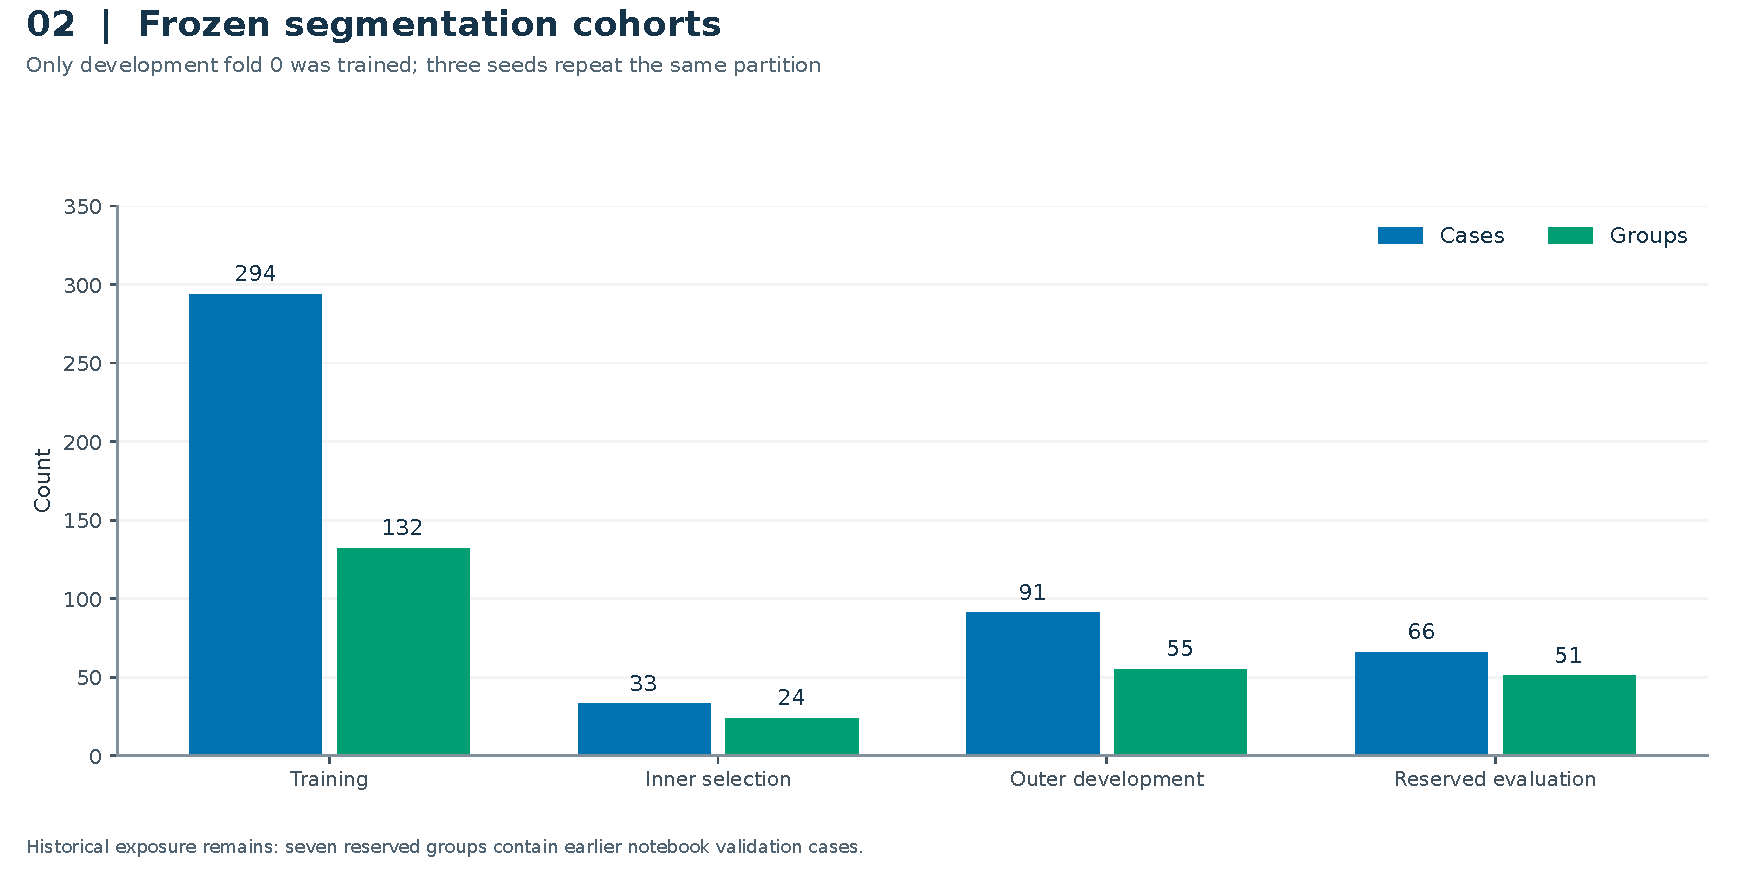
\includegraphics[width=\columnwidth]{figures/fig02_segmentation_cohorts.pdf}
\caption{Executed fold-0 roles and the reserved cohort after conservative similarity grouping; the 15-group historical-sensitivity subset is nested inside the reserved cohort.}
\label{fig:cohorts}
\end{figure}

